%%%%%%%%%%%%%%%%%%%%%%%%%%%%%%%%%%%%%%%%%%%%%%%%%%%%%%%%%%%%%%%%%%%%%%%%
% Created 2020-09-30 Wed 15:22
% Intended LaTeX compiler: pdflatex
\documentclass[10pt,t]{beamer}
\usepackage[utf8]{inputenc}
\usepackage[T1]{fontenc}
\usepackage{graphicx}
\usepackage{grffile}
\usepackage{longtable}
\usepackage{wrapfig}
\usepackage{rotating}
\usepackage{amsmath}
\usepackage{textcomp}
\usepackage{amssymb}
\usepackage{capt-of}
\usepackage{hyperref}
\usetheme{default}
%\usepackage{scrextend}
%\usepackage{lipsum}

\author{S. Machado}
\date{\today}
\title{\large AIRS Climate Temperature and Humidity 19-Year Trends: Is Relative Humidity Changing}
\subtitle{\footnotesize{AIRS Virtual Science Team Meeting}}
\date{\vspace{0.1in}\footnotesize{October 26-28, 2021 \vfill}}
\author{Sergio DeSouza-Machado\inst{2}, L. Larrabee Strow\inst{1,2}, \newline 
Howard Motteler\inst{2}, Ryan Kramer \inst{2,3}  and  Chris Hepplewhite\inst{2}}
\institute[UMBC]{\inst{1} UMBC Physics Dept. \and \inst{2}UMBC JCET \and \inst{3}NASA Goddard}
\input beamer_setup
\usetheme{metropolis}
\metroset{titleformat title=allcaps}
\renewcommand{\UrlFont}{\small\tt}
\renewcommand*{\UrlFont}{\footnotesize}
\tolerance=1000
\begin{document}

\maketitle

%%%%%%%%%%%%%%%%%%%%%%%%%%%%%%%%%%%%%%%%%%%%%%%%%%%%%%%%%%%%%%%%%%%%%%%%
\begin{frame}[shrink=2]{Outline}
%\begin{frame}{Outline}

\begin{block}{Motivation:}
\begin{itemize}
\item Create long-term climate-quality geophysical trends from AIRS/CrIS
\item Minimize uncertanties due to:
\begin{itemize}
\item Absolute calibration
\item RTA bias errors
\item A-priori information
\end{itemize}
\end{itemize}
\end{block}

\begin{block}{Approach:}
\begin{itemize}
\item Long-term: Retrieval geophysical anomalies \emph{directly} from radiance anomalies to enhance climate accuracy
\item This talk:
\begin{itemize}
\item By-pass anomaly retrievals (time-series) and focus on 19-year linear trend retrievals directly from radiance linear trends.
\end{itemize}
\item Trends presented here will serve as closure tests for future anomaly trend retrievals
\end{itemize}
\end{block}

\begin{block}{Feedbacks:}
\begin{itemize}
\item Use retrieved linear trends to estimate climate feedbacks
\end{itemize}
\end{block}

\end{frame}

%%%%%%%%%%%%%%%%%%%%%%%%%%%%%%%%%%%%%%%%%%%%%%%%%%%%%%%%%%%%%%%%%%%%%%%%

\begin{frame}{OEM Retrievals}
\begin{block}{}
\begin{itemize}

\item {\large Use trends from hottest (clearest) obs and/or the
      mean (allsky) observations}
\item Use 20 layers and zero \emph{a-priori}
\item fix trace gases (CO2, N2O, CH4) to ESRL rates; retrieve T(z),WV(z),O3(z),surf temp trends
\item Compare against following datasets, starting Sept 2002
  \begin{itemize}
  \item ERA5 monthly (ERA-I daily stopped August 2019)
  \item AIRS3 L3 monthly
  \item CMIP6 : historical runs all forcings, monthly to Aug 2014
  \end{itemize}
\item Timings on UMBC HPC cluster
  \begin{itemize}
    \item All the hard work in tiling 18 years of AIRS data done, now all we do is add on a month or so at a time
    \item Run off trends/anomalies (day or so)
    \item 64 $\times$ 72 trend retrievals $\rightarrow$ 15 mins, 64 zonal averages $\rightarrow$ 1 min
    \item compare to re-processing AIRS L2 or L3 ....
  \end{itemize}
\end{itemize}
\end{block}
\end{frame}

%%%%%%%%%%%%%%%%%%%%%%%%%%%%%%%%%%%%%%%%%%%%%%%%%%%%%%%%%%%%%%%%%%%%%%%%
\begin{frame}{OLR in the Far-IR}
\begin{block}{}

\vspace{-0.1in}
\begin{columns}

\begin{column}{0.55\columnwidth}
\begin{block}{}
\vspace{-0.1in}
\begin{center}
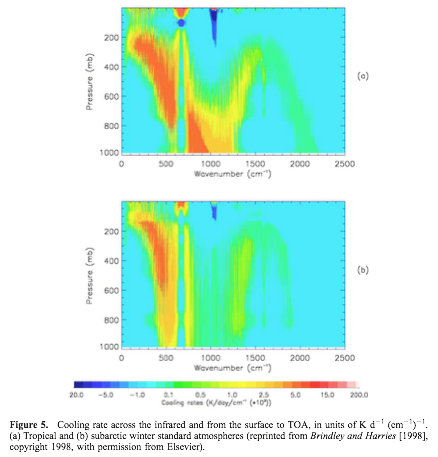
\includegraphics[width=\linewidth]{image_spectralOLR.png}
\end{center}
\end{block}
\end{column}

\begin{column}{0.55\columnwidth}
\begin{block}{}
\begin{itemize}
\item Far-IR WV emission dominates atmospheric cooling, esp. in descending tropical regions
\item AIRS observed mid-IR WV has sensitivity where (WV) OLR is large in far-IR
\item Allows computation of feedbacks from AIRS retrievals using computed OLR driven by mid-IR WV retrievals
\end{itemize}
\end{block}
\end{column}

\end{columns}

\end{block}
\end{frame}

%%%%%%%%%%%%%%%%%%%%%%%%%%%%%%%%%%%%%%%%%%%%%%%%%%%%%%%%%%%%%%%%%%%%%%%%

\begin{frame}{Night ALL Spectral Rates}

% \textcolor{red}{Green curve is very similar to MEAN AIRS obs trends shown by Larrabee in previous talk!}

\begin{center}
\includegraphics[width=0.95\linewidth]{Figs_STMOct2021/spectral_all_N_ratesV2.png}
\end{center}
\end{frame}


\begin{frame}{Simulated tropical $dBT(\nu)/dt$}

\vspace{-0.1in}
\begin{columns}

\begin{column}{0.75\columnwidth}
\begin{block}{}
\vspace{-0.1in}
\begin{center}
\includegraphics[width=0.975\linewidth]{Figs_STMOct2021/delta_BT_with_WVv3.pdf}
\end{center}
\end{block}
\end{column}

\begin{column}{0.35\columnwidth}
\begin{block}{}

\begin{itemize}
\item Realistic dT(z)/dt, dCO2/dt = 2.2 ppm/yr
\item WVfrac changes to (a) keep RH constant, or \newline (b) reduce RH
\end{itemize}
\end{block}
\end{column}

\end{columns}

\end{frame}

%%%%%%%%%%%%%%%%%%%%%%%%%%%%%%%%%%%%%%%%%%%%%%%%%%%%%%%%%%%%%%%%%%%%%%%%

\begin{frame}{Is $\delta$ RH = 0}


{\bf Climate Change 2007: Working Group I: The Physical Science Basis} \newline
https://archive.ipcc.ch/publications\_and\_data/ar4/wg1/en/ch8s8-6-3-1.html \newline

Understanding processes determining the distribution and variability
in RH is therefore central to understanding of the water vapour-lapse
rate feedback. \emph{To a first approximation, GCM simulations indeed
maintain a roughly unchanged distribution of RH under greenhouse gas
forcing. More precisely, a small but widespread RH decrease in GCM
simulations typically reduces feedback strength slightly compared with
a constant RH response} (Colman, 2004; Soden and Held, 2006; Figure
8.14).

\end{frame}
%%%%%%%%%%%%%%%%%%%%%%%%%%%%%%%%%%%%%%%%%%%%%%%%%%%%%%%%%%%%%%%%%%%%%%%%

\begin{frame}{Surface Temperature Trends K/yr}
\begin{footnotesize}
\begin{itemize}
\item May 2021 STM excellent agreement with GISTEMP, HADCRU4
\item They do not see AIRS L3 cooling in the Antartic
\item allsky trends $\sim$ hottest trends on average, much more spatial variation
\end{itemize}
\end{footnotesize}
\begin{center}
\includegraphics[width=0.925\linewidth]{Figs_STMOct2021/skt_rates_tiled.png}
\end{center}
\end{frame}

\begin{frame}{Night Land Atmospheric temperature Trends K/yr}
\begin{center}
\includegraphics[width=0.95\linewidth]{Figs_STMOct2021/tiled_land_N_T_trend.png}
\end{center}
\end{frame}

\begin{frame}{Night Ocean Atmospheric temperature Trends K/yr}
\begin{center}
\includegraphics[width=0.95\linewidth]{Figs_STMOct2021/tiled_ocean_N_T_trend.png}
\end{center}
\end{frame}

%\begin{frame}{Night All} : dT/dt}
%\begin{center}
%\includegraphics[width=0.95\linewidth]{Figs_STMOct2021/tiled_all_N_T_trend.png}
%\end{center}
%\end{frame}



\begin{frame}{Night Land dWVfrac/dt 1/yr}
\begin{center}
\includegraphics[width=0.95\linewidth]{Figs_STMOct2021/tiled_land_N_WVfrac_trend.png}
\end{center}
\end{frame}

\begin{frame}{Night Ocean dWVfrac/dt 1/yr}
\begin{center}
\includegraphics[width=0.95\linewidth]{Figs_STMOct2021/tiled_ocean_N_WVfrac_trend.png}
\end{center}
\end{frame}

%\begin{frame}{Night All} : dWVfrac/dt}
%\begin{center}
%\includegraphics[width=0.95\linewidth]{Figs_STMOct2021/tiled_all_N_WVfrac_trend.png}
%\end{center}
%\end{frame}

\begin{frame}{Night Land : dRH/dt percent/yr}
\begin{center}
\includegraphics[width=0.95\linewidth]{Figs_STMOct2021/tiled_land_N_RH_trend.png}
\end{center}
\end{frame}

\begin{frame}{Night Ocean : dRH/dt percent/year}
\begin{center}
\includegraphics[width=0.95\linewidth]{Figs_STMOct2021/tiled_ocean_N_RH_trend.png}
\end{center}
\end{frame}

%\begin{frame}{Night All} : dRH/dt}
%\begin{center}
%\includegraphics[width=0.95\linewidth]{Figs_STMOct2021/tiled_all_N_RH_trend.png}
%\end{center}
%\end{frame}

\begin{frame}{Night Land}
\begin{center}
\includegraphics[width=0.95\linewidth,height=0.875\textheight]{Figs_STMOct2021//tiled_land_N_T_RH_WVfracrates.png}
\end{center}
\end{frame}

\begin{frame}{Night Ocean}
\begin{center}
\includegraphics[width=0.95\linewidth,height=0.875\textheight]{Figs_STMOct2021//tiled_ocean_N_T_RH_WVfracrates.png}
\end{center}
\end{frame}

%\begin{frame}{Night All}}
%\label{all:trends}
%\begin{center}
%\includegraphics[width=0.95\linewidth,height=0.875\textheight]{Figs_STMOct2021//tiled_all_N_T_RH_WVfracrates.png}
%\end{center}
%\end{frame}

%%%%%%%%%%%%%%%%%%%%%%%%%%%%%%%%%%%%%%%%%%%%%%%%%%%%%%%%%%%%%%%%%%%%%%%%
\begin{frame}{Night All : Spectral closure with unc}
\begin{footnotesize}
Obs uncertainty : fitting the 16 day avg data, has all inter-anual variability \newline
Retrieval+Model uncertainty : unc in geophysical trends $\rightarrow$ spectra \newline
\end{footnotesize}
\begin{center}
%\includegraphics[width=0.95\linewidth,height=0.625\textheight]{~/MATLABCODE/oem_pkg_run/AIRS_gridded_STM_May2021_trendsonlyCLR_zonalavg/spectral_plot_with_unc2.pdf}
\includegraphics[width=0.95\linewidth,height=0.625\textheight]{~/MATLABCODE/oem_pkg_run/AIRS_gridded_STM_May2021_trendsonlyCLR/spectral_plot_with_unc2_64x72.pdf}
\end{center}
\end{frame}
%%%%%%%%%%%%%%%%%%%%%%%%%%%%%%%%%%%%%%%%%%%%%%%%%%%%%%%%%%%%%%%%%%%%%%%%

\begin{frame}{Feedback Parameters}

{\small 
Use one sided OLR clear sky changes from ecRad (R. Hogan, ECMWF) and equations from 
Jevanjee, Koll, Lutsko, ``Simpson's Law and the Spectral Cancellation of Climate Feedbacks'', GRL 2020}

\vspace{-0.25in}
\begin{columns}

\begin{column}{0.55\columnwidth}
\begin{block}{}
\vspace{-0.1in}
\begin{center}
\includegraphics[width=0.975\linewidth]{Figs_STMOct2021//tiled_feedbackparams.pdf}
\end{center}
\end{block}
\end{column}

\begin{column}{0.55\columnwidth}
\begin{block}{}
\begin{itemize}
\item $\lambda = -\frac{d(OLR(xf)-OLR(x0))}{d(ST)}$
\item Preliminary work
%\item Used same underlying X0 geophysical (unperturbed state)
%\item Perturb using dST/dt,dT(z)/dt,dWVfrac/dt $\rightarrow \lambda$
\item Planck : IPCC $\sim$ -3.3 W/m2/K
\item SKT : use window region Planck!
\item WV and Lapse feedback : UMBC and AIRS L3 are obs, quite similar!
\end{itemize}
\end{block}
\end{column}

\end{columns}
\end{frame}

\begin{frame}{Feedback Values (W/m2/K)}

Notable differences between \emph{Observations} versus Models

\begin{center}
\begin{tabular}{ c c c c c}
\hline
        &   Planck   &     Lapse    &      WV    &        SKT  \\
\hline
\emph{UMBC}    & -3.89  &   \emph{0.93}   &   \emph{0.27} &   -1.18 \\
\emph{AIRS v7} & -3.89  &   \emph{1.26}   &   \emph{0.46} &   -1.18 \\
ERA5    & -3.89  &   0.13   &   1.13 &   -1.18 \\
CMIP6   & -3.89  &  -0.21   &   1.95 &   -1.18 \\
\hline
\hline
\emph{AIRS v6} & & \emph{0.77} & \emph{1.05} & \\
\emph{AIRS v7} & & \emph{0.67} & \emph{0.73} & \\
MERRA2  & & -0.03 & 1.61 & \\
ERA5    & & -0.46 & 1.83 & \\
\hline
\end{tabular}
\end{center}
Haozhe He, 12 pm talk \emph{Evaluating Observational Constraints on Intermodel Spread in
Cloud, Temperature and Humidity Feedbacks}

\end{frame}

%%%%%%%%%%%%%%%%%%%%%%%%%%%%%%%%%%%%%%%%%%%%%%%%%%%%%%%%%%%%%%%%%%%%%%%%

\begin{frame}{Conclusions}

\begin{block}{Conclusions}
\begin{itemize}

\item \textcolor{red}{Zero \emph{a-priori}} for thermodynamic trends (19 years of AIRS data)

\item \textcolor{red}{Spectral closure indicative that UMBC retrievals are correct}
\begin{itemize}
\item same results using trends from clearest obs (4608 tiles), clearest obs (64 zonal averages), mean obs (4608 tiles)
\item used results for deriving feedbacks parameters
\end{itemize}

\item ST (not shown) and T(z,lat) trends 
%\begin{localsize}{8}
\begin{itemize}
\item are approximately same for UMBC, AIRS L3, ERA5; CMIP6 shows more warming in N. Polar
\item more warming over ocean than land
\end{itemize}
%\end{localsize}

\item WVfrac(z,lat) and RH(z,lat) trends 
%\begin{localsize}{8}
\begin{itemize}
\item UMBC shows tiniest increases, not large enough to offset T increase, so RH decreases overall
\item So does AIRS L3!
\item ERA5 and CMIP6 seem to imply that RH is $\sim$ constant
\end{itemize}
%\end{localsize}

\item Feedback parameters from obs different from models
\end{itemize}
\end{block}

\end{frame}
\end{document}
%%%%%%%%%%%%%%%%%%%%%%%%%%%%%%%%%%%%%%%%%%%%%%%%%%%%%%%%%%%%%%%%%%%%%%%%
